\chapter{Búsqueda de SUSY con fotones y Higgs en el estado final con producción fuerte}
% \addcontentsline{toc}{chapter}{Búsqueda de SUSY con fotones y Higgs en el estado final}
\chaptermark{Búsqueda de SUSY con fotones y Higgs en el estado final con producción fuerte}


El análisis para el cual está orientada esta Tesis consiste en la búsqueda de Supersimetría en eventos con un fotón aislado muy energético, jets y gran cantidad de energía faltante en estado final \cite{Alonso:2147473,ATLAS:2016fks,Collaboration:2198651}. La estrategia general de la búsqueda consiste en el conteo del número de eventos observado en exceso sobre el SM en una cierta región del espacio de observables rica en eventos de la señal considerada.


\section{Identificación de eventos de fondo}

Para un correcto procedimiento, es necesario conocer los procesos del SM que tengan un estado final equivalente a de la señal buscada. Estos eventos toman el rol de fondo en el contexto de un análisis de búsqueda de SUSY. Para este análisis, son procesos que tienen un fotón, jets y energía faltante en el estado final, y pueden dividirse en varias categorías. Por un lado, los procesos que dan lugar a eventos con un fotón y energía faltante real, es decir, los que se llaman fondos irreducibles. Estos son:

\begin{itemize}

	\item $Z(\rightarrow \nu\nu)$ + $\gamma$

	\item $W (\rightarrow l\nu)$ + $\gamma$

	\item $t \overline{t}$ + $\gamma$

\end{itemize}

También es posible que, aunque el proceso no tenga fotones en el estado final, un electrón o un jet sean identificados como un fotón, dando lugar a un estado final idéntico al buscado. En esta categoría están:

\begin{itemize}

	\item $W (\rightarrow l\nu)$ + jets

	\item $Z (\rightarrow \nu\nu)$ + jets

	\item $t \overline{t}$

	\item $WW$, $ZZ$, $WZ$

\end{itemize}

Y por último, también puede haber procesos que a pesar de no generar energía faltante real, poseen lo que se denomina energía faltante instrumental, proveniente generalmente de la incorrecta reconstrucción de la energía de los jets. De esta manera, pueden dar lugar a eventos con el estado final de interés, los procesos QCD:

\begin{itemize}

	\item $\gamma$ + jets

	\item multijet, con alguno de los jets identificado como fotón

	\item $Z(\rightarrow ll)$ + jets, donde un leptón o un jet es identificado como un fotón

\end{itemize}


\section{Muestras a partir de simulaciones de Monte Carlo}

Muestras de señal de SUSY y fondos del SM fueron simulados
utilziando generadores de Monte Carlo (MC) dedicados a $\sqrt{s} = 13 \tev$.
Las muestras de señal de SUSY se realizaron mediante una simulación rápida \textsc{ATLFAST-II} \cite{Richter-Was:683751} del detector ATLAS, mientras que las muestras de fondo SM realizaron con una simulación completa basada en \textsc{Geant4}\cite{Geant4} del detector ATLAS, y reconstruido con los mismos
algoritmos utilizados en los datos. Un peso evento a evento es aplicado
a todas las muestras de MC para modelar las condiciones del detector de la muestra de datos bajo estudio,
haciendo coincidir la distribución simulada del número de colisiones inelásticas $pp$ por cruce de haces con el observado en los datos.

Las simulaciones se corrigen a su vez con factores de escala de eficiencia.
y correciones en la escala de energía de fotones, leptones y
jets, para describir mejor los datos. Las muestras se generaron con un
distribución de pileup esperada, denominadas MC16a, MC16d y MC16e para el conjunto de datos 2015-2016, 2017 y
2018 respectivamente, con un peso adicional para igualar
el perfil de interacción real de los datos. 


\subsection{Muestras de fondo}

Varios procesos del SM pueden imitar una señal SUSY con fotones, jets y
energía transversa faltante. Estos surgen de eventos con
fotones reales o eventos en los que un electrón o un jet es
identificado erróneamente como un fotón. Es esperado que la primera sea principalmente
de eventos en los que se produce un bosón  $W$, $Z$ o un par $t\bar{t}$ en
asociación con al menos un fotón real, decayendo subsecuentemente a neutrino prodciendo importantes cantidades de \met. 
Estos fondos son denominados $W\gamma$, $W\gamma\gamma$, $Z\gamma$, $Z\gamma\gamma$ y
$t\bar{t}\gamma$. Los eventos con fotones reales también pueden contribuir
al fondo cuando \met surge de una reconstrucción instrumental incorrecta de la energía. Los fondos de $W\gamma$, $t\bar{t}\gamma$ y $\gamma + $jets
se estiman normalizando la muestra de MC correspondiente para que coincida con el
número de eventos observados en las regiones de control correspondientes, enriqeucidas en el fondo dado
y cinemáticamente similares a las
regiones de señal. Contribuciones más pequeñas de $\gamma\gamma$,
$W\gamma\gamma$, $Z\gamma$ y $Z\gamma\gamma$ son estimados
directamente de las simulaciones de MC. La contaminación
a partir de fondos de fotones falsos debido a la identificación errónea de electrones y jets
que surgen de $W$ + jets, $Z$ + jets, \ttbar o eventos de multijets, se estiman con una técnica basada en datos que se explica en las siguientes secciones.
La Tabla \ref{tab:background} resume las principales fuentes de fondo anteriormente mencionadas.

\begin{table}[ht!]
\centering
        \begin{tabular}{|c|c|c|}
      \hline
      & \textbf{Real {\met}} & \textbf{Instrumental {\met}} \\
        \hline
        \textbf{Real photon} &
      \begin{tabular}[c]{@{}c@{}}
        $Z(\nu\nu)\gamma$, $W\gamma$ \\
        $t\bar{t}\gamma$, $Z(\nu\nu)\gamma\gamma$, $W\gamma\gamma$ \\
      \end{tabular}
      &    $\gamma+$jets, $\gamma\gamma$, $Z(ll)\gamma$, $Z(ll)\gamma\gamma$  \\
      \hline
      \textbf{Fake photons}    &
      \begin{tabular}[c]{@{}c@{}}
        $W$+jets, $Z(\nu\nu)+$jets \\
        $t\bar{t}$ \\
      \end{tabular}
      &     multijet, $Z(ll)+$jets \\
      \hline
      \end{tabular}
\caption{Procesos del SM que constribuyen al fondo.}
 \label{tab:background}
\end{table} 

\subsection{Muestras de señal}
\label{sec:signal}


El presente análisis está motivado por la presencia de neutralinos mezcla de bino-higgsino
mezcla con un estado final predicho por el modelo de General Gauge Mediation
compuesto de al menos un
fotón, jets y alto \met. El componente bino del neutralino más liviano se acopla tanto al fotón como al bosón $Z$. El gluino es
considerada como la única espartícula de color relevante para establecer un
límite conservador en la masa de gluino.

Todas las masas de los squark se establecen en 5 $\tev$. Esto da como resultado una producción de procsos SUSY a través de la creación de pares de gluinos, cada uno de los cuales
que decae posteriormente a través de un squark virtual (los 12 estados de sabor de los squarks se consideran completamente degenerados) a un
pares quark-antiquark más el neutralino NLSP.

Otros parámetros del modelo se establecen en $M_ {2} = 3\ \tev$, $ \tan{\beta} = 1.5$ y $m_{\tilde{G}} = 1$ eV.
Todos los términos de acoplamiento trilineal se establecen en cero y las masas de sleptons se establecen en 5 \tev. El bosón de Higgs está en el régimen de desacoplamiento con $m_{A} = 2\ \tev $ y
$m_{h} = 125\ \gev$, valor medido recientemente en el LHC para el
Bosón de Higgs del SM \cite{Aad:2015zhl}. En escenarios SUSY \textit{gauge mediated}
existen varios mecanismos \cite{Craig:2011yk, Auzzi:2011eu, Csaki:2012fh, Larsen:2012rq, Craig:2012hc} para generar una masa de bosón de Higgs como este valor observado, sin cambiar el
fenomenología de los modelos aquí considerados. Además $c\tau_{\mathrm{NLSP}}
<0.1$ mm se estableció para asegurar que el neutralino decaiga rápidamente y el
decaimiento directo del gluino está prohibido fijando $BR(\gluino \to \gravino g) = 0$.

Como $M_1$ y $\mu$ determinan la masa neutralino más ligera, están relacionados
de tal manera que las fracciones de decaimiento del \ninoone\ sean aproximadamente
constante, resultando en $\text{BR} (\ninoone \to \gamma \gravino) \sim 50 \%$,
$\text{BR} (\ninoone \to Z\gravino) \sim 0 \% $ y $ \text{BR} (\ninoone \to h
\gravino) \sim 50 \%$, números que varían en $\pm 1 \%$ para todas las muestras.
% como se muestra en la Figura \ ref {fig: br_n1_X}.

Vale la pena señalar que $\sim 25 \%$ de eventos tendrán dos fotones en el estado final,
por lo que se realiza una búsqueda inclusiva que requiera al menos un
$\gamma$, más dos \gravino\ en el estado final.

El valor de $\mu$ también debe ser negativo para no favorecer los decaimientos al bosón de $Z$, lo que daría lugar a un estado final que es cubierto por otro análisis. Esto deja $M_3$ y $\mu$ como los únicos dos parámetros libres del modelo, que son variados desde $150\ \gev<m_{\ninoone}<(m_{\ gluino} - 50) \ \ gev $ y $1200\ \gev<m_{\gluino}<2400\ \gev$
con $m_{\ninoone}<m_{\gluino}$.

% Para hacer coincidir las masas de gluinos correspondientes a los archivos LHE disponibles, no se tienen en cuenta las correcciones radiativas, lo que implica que
% Las masas de gluino ahora coinciden con los valores del parámetro M3 (este no fue el caso
% para la producción anterior de MC15).


Los puntos de señal generados se resumen en la Figura \ref{fig:signal_grid}. Consta de 81 puntos de produccion fuerte ($\gluino\gluino$) generados con $10000$ eventos cada uno.


Se calcularon el espectro de masas completo, las fracciones de decaimiento del gluino y neutralino y los anchos de desintegración de este conjunto de puntos utilizando SUSPECT v2.43 \cite{Djouadi2007426}, SDECAY v1.5 \cite{Muhlleitner:2004mka} y HDECAY v3.4 \cite{Djouadi:1997yw},
ejecutados como parte del paquete SUSYHIT v1.5a \cite{Djouadi:2006bz}.
Como ejemplo, la \ref{fig:mass_spectra} muestra el espectro de masas para uno de los puntos en la cuadrícula de señales GGM, con ($M_3$, $\mu$) = (1600 {\gev}, 650 \gev). 

\begin{figure}
  \centering
  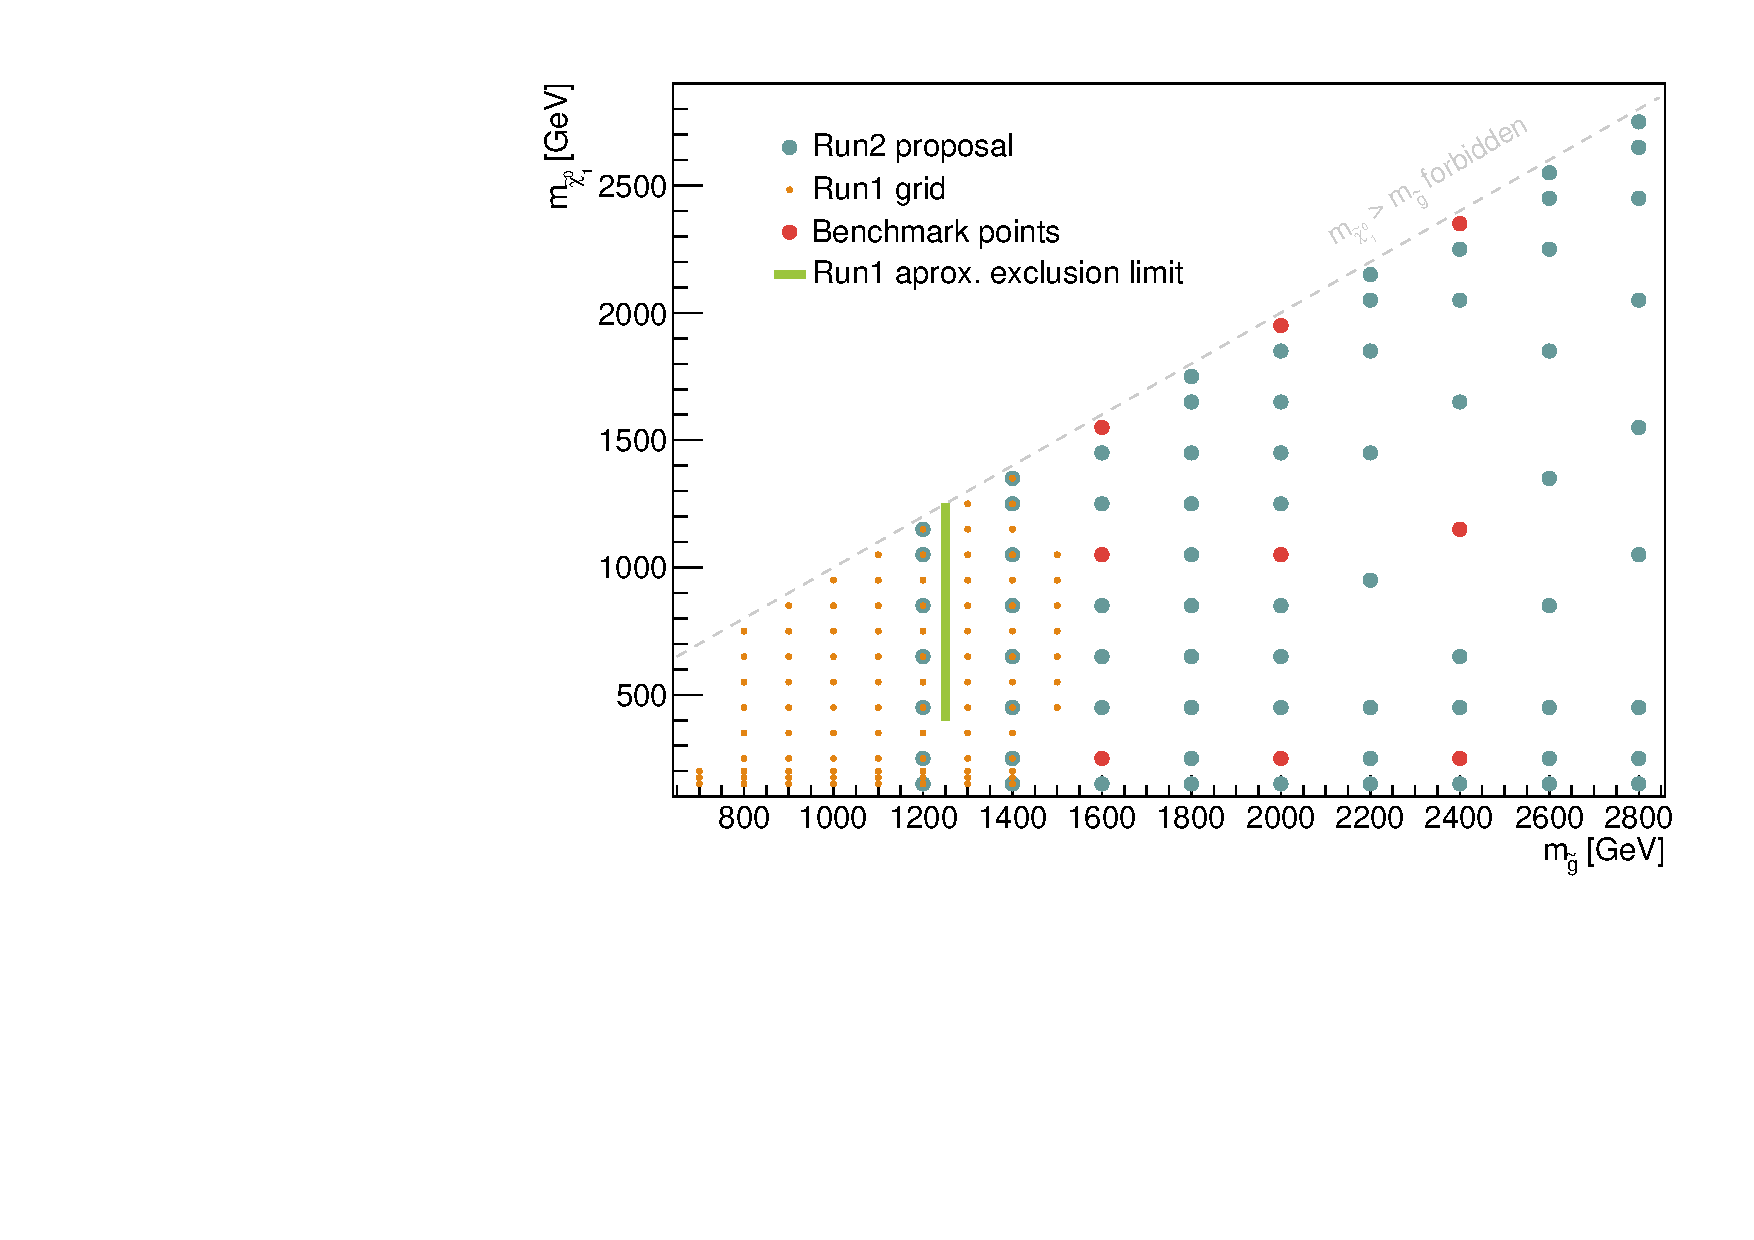
\includegraphics[width=0.7\textwidth]{images/phb_grid.pdf}
  \caption{Grid de puntos de señal simulados.}
  \label{fig:signal_grid}
\end{figure}

\begin{figure}
  \centering
  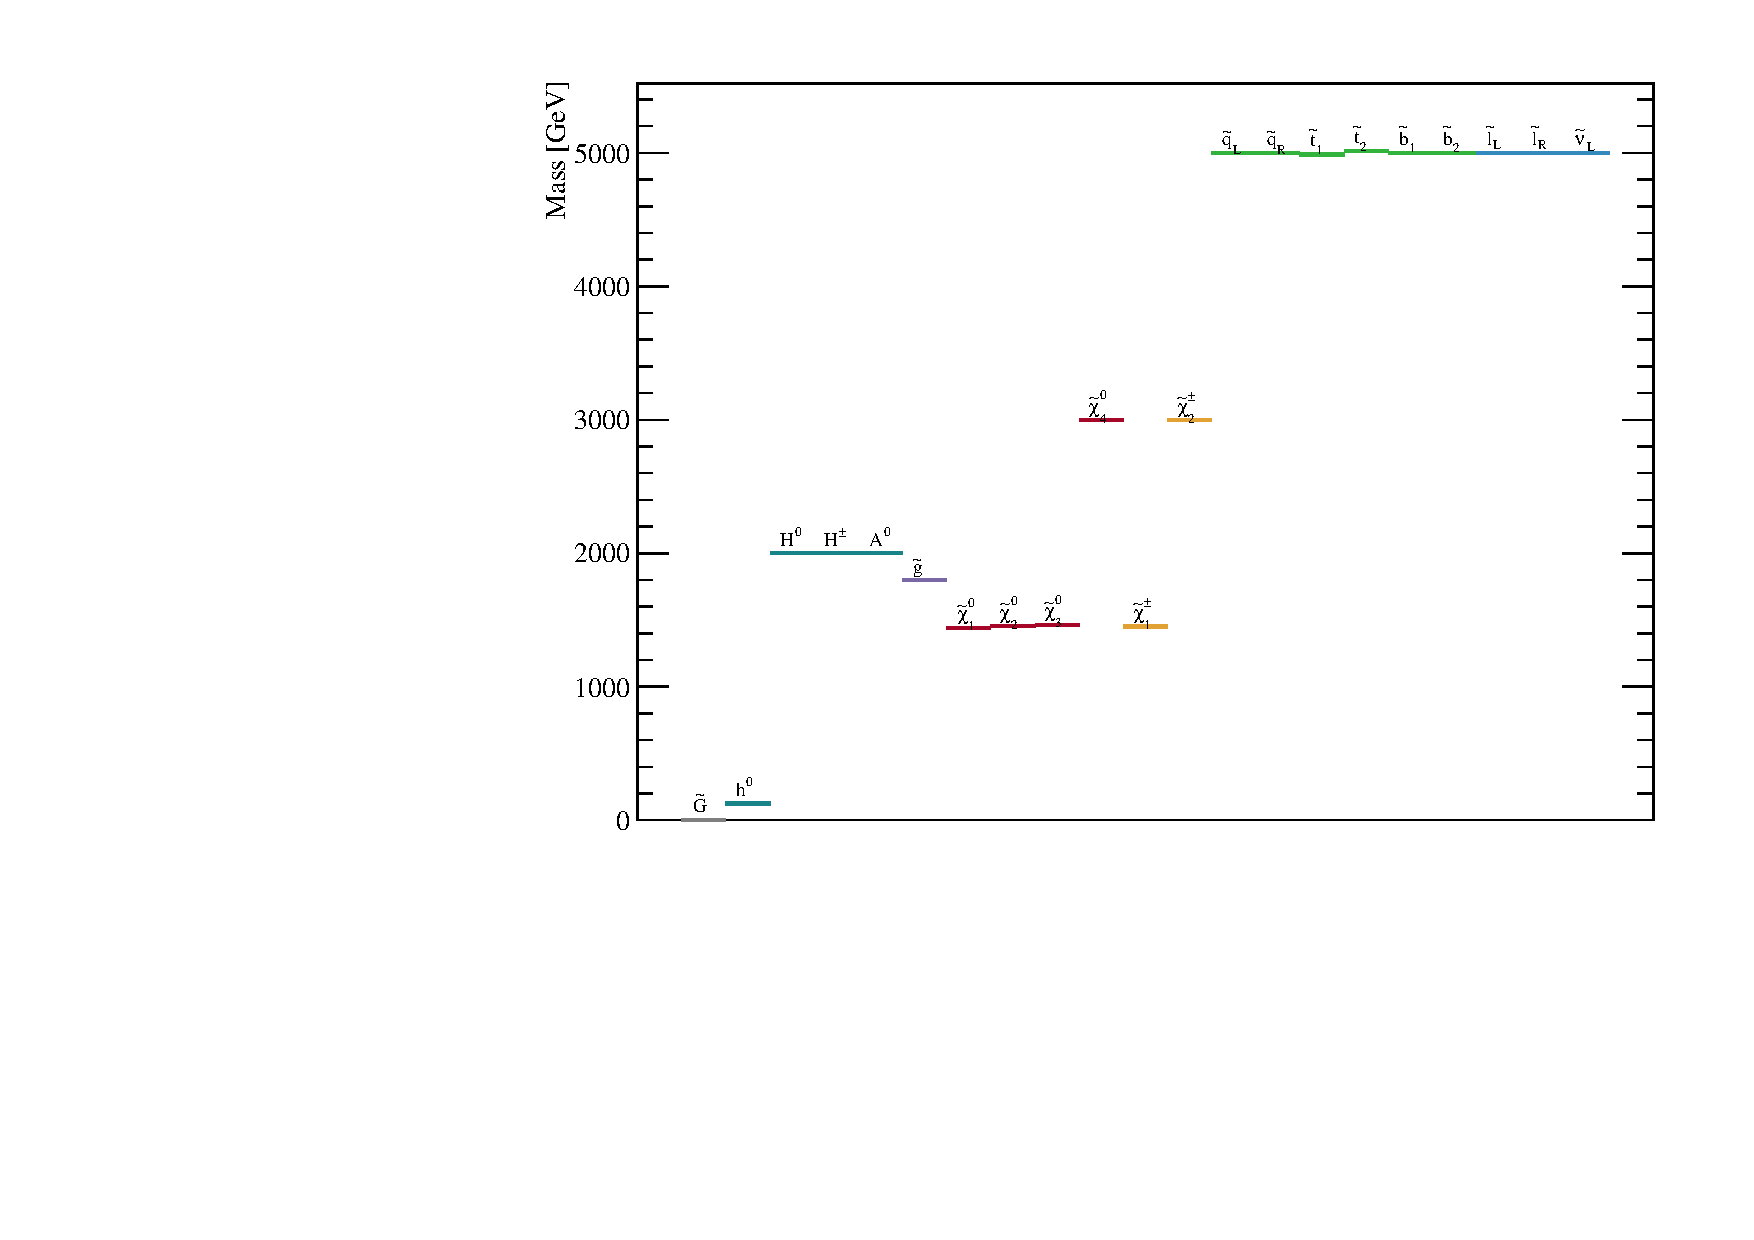
\includegraphics[width=0.7\textwidth]{images/phb_mass_spectrum.pdf}
  \caption{Espectro de masas para el punto de señal ($M_3$, $\mu$) = (1600 {\gev}, 650 \gev).}
  \label{fig:mass_spectra}
\end{figure}

\section{Selección de eventos de señal}

El análisis está diseñado para comparar el número de eventos observados en tres regiones de señal para la producción fuerte (denominadas SRL, SRM y SRH) con las predicciones de los procesos de SM.
La SRL apunta al espacio de fase con grandes diferencias de masa entre el gluino y el neutralino, lo que resulta en eventos caracterizados por una gran multiplicidad de jets y actividad hadrónica, pero momento transverso faltante moderado. La región de señal SRH está optimizada para los escenarios comprimidos, cerca de la diagonal en el plano de masa gluino-neutralino, dando eventos con un alto momento transverso faltante, fotones con \pt\ más alto y una multiplicidad de jets y actividad hadrónica más bajas. Finalmente, la región SRM se define para el espacio de fase intermedia entre SRL y SRH.

Dada la gran masa de gluinos producidos en el modelo GGM explorado, se espera que el momento transversal visible total sea grande. Esto da como resultado un valor grande para la variable \HT, definida como la suma escalar de los momentos transversales de todos los jets de señal individuales y el fotón principal en el estado final.
La selección de eventos de señal incluye un requisito un \HT \ y \met.
En SRL, SRM y SRH, se requiere que los eventos contengan al menos un fotón aislado con $\ET> 145$, $>300 $ o $>400\ \gev$, respectivamente, y cero leptones para eliminar los eventos SM que contengan $ V\gamma$ donde el bosón del vector decae leptónicamente. Además, se requieren más de cuatro jets en SRL y SRM, mientras que se requieren más de dos jets en SRH.

En eventos caracterizados por elevado \met\ reconstruidos sin una contribución significativa de partículas que no interactuantes o que surge de fuentes instrumentales y objetos físicos mal reconstruidos, el vector de momento transverso faltante tiende a
estar alineado con el fotón o con uno de los dos jets principales. Una selección basada en la separación angular entre estos objetos y el vector \met\ ($\dphijetmet$ y $\dphigammet$) proporciona una gran supresión de estos procesos de fondo.

Las señales de SUSY consideradas en este análisis se caracterizan por
eventos con alta multiplicdad de jets en una amplia región del espacio de parámetros. Los jets secundarios son comparativamente más duros que los de los eventos de fondo SM. Como consecuencia, para procesos de señal con jets duros, \rtf\ (definido como la suma escalar de \pt\ para los cuatro jets de \pt\ más alto, dividido la suma escalar del \pt\ de todos los jets de señal) toma valores inferiores a uno, mientras que para el fondo SM con menos jets y más suaves, \ \rtf\ suele estar más cerca de la unidad \cite{SUSY-2016-27}.
No se aplica una selección de \rtf\ para SRH debido al menor número de jets en esta región.

La selección de eventos para todas las regiones de señales se resume en la Tabla \ref{tab:sr_selection}. 

\begin{table}[ht!]
  \centering
  \begin{tabular}{lrrr}
    \hline
    \hline
                                                    &        SRL    &       SRM     &         SRH \\
      \hline
      $\nph$                        &        $\ge1$ &        $\ge1$ &        $\ge1$ \\
      $\ptph$                 &  $>145\ \gev$ &  $>300\ \gev$ &  $>400\ \gev$ \\
      $\nlep$                        &             0 &             0 &             0 \\
      $\njet$                           &       $\ge 5$ &       $\ge 5$ &       $\ge 3$ \\
      $\dphijetmet$                &        $>0.4$ &        $>0.4$ &        $>0.4$ \\
      $\dphigammet$                    &        $>0.4$ &        $>0.4$ &        $>0.4$ \\
      $\met$                                       &  $>250\ \gev$ &  $>300\ \gev$ &  $>600\ \gev$ \\
      $\HT$                                         & $>2000\ \gev$ & $>1600\ \gev$ & $>1600\ \gev$ \\
      $\rtf$                            &       $<0.90$ &       $<0.90$ &             - \\
      \hline
      \hline
    \end{tabular}
  \caption{Selección para las tres regiones de señal.}
  \label{tab:sr_selection}
\end{table}



\section{Regiones de control y validación}

Se espera que las contribuciones de fondo dominantes del SM en las SR sean de la
producción de $W \gamma$ y \ttbarph\, seguida de una producción de fotones con \met instrumental. Estas tres contribuciones se determinan utilizando simulaciones de MC restringidas por eventos observados en regiones de control dedicadas a través de la estimación de factores de normalización. Las fuentes de fondo más pequeñas,
$ W \gamma \gamma $, $ Z \gamma $, $ Z \gamma \gamma $ y $ \gamma \gamma $, se obtienen
directamente de MC.

Las regiones de control denominadas como CRW, CRT y CRQ se utilizan para obtener el MC
normalización para los eventos $ W \gamma $, \ttbarph y QCD \phj\, respectivamente.
Los criterios de selección para las CR asociadas con las SR se presentan en la Tabla \ref{tab:CR_VR_selection}. Las CR están diseñadas para ser ortogonales pero aún cinemáticamente similares a las SR, y que favorezcan el proceso de fondo de interés, con una contaminación de señal insignificante.

La selección para la CRQ se define a partir de las SRs pero
aplicando un requisito en \met\ más bajo ($> 100\ \gev $), una selección \HT\ similar
y $ \dphijetmet$ invertido, aplicados para aumentar la fracción de
\phj\ en la muestra de control.

La región CRW se define al requerir un fotón, un leptón y $ 100\ \gev <\met <200 \ \gev $. Se aplica un requisito de veto de $b$-jets para reducir la contaminación de \ttbarph.

La región CRT se define al requerir un fotón, un leptón, jets y $ 50 \ \gev <\met <200 \ \gev $. Se requieren al menos dos jets etiquetados con $b$ para aumentar la pureza de la población de eventos de \ttbarph. También se aplican requisitos más flexibles en ambos casos para aumentar los rendimientos. No se aplica ningún requisito en \rtf por la misma razón. Se aplica un requisito de \met máximo para reducir la contaminación de la señal.

Se utiliza un conjunto adicional de Regiones de validación (VR) para verificar
los resultados del procedimiento de estimación de anteriores. Fueron diseñadas para encontrarse
cinemáticamente entre las regiones de señal y las regiones de control, pero con uno o más criterios
invertido o modificado para reducir una posible contaminación de la señal. Las regiones VRL son
diseñado para enriquecer los fondos $ W \gamma $ y $ \ttbarph $. No se aplica ningún requisito de $ b $-jets,
por lo que se espera la contribución de ambos procesos. Las cuatro regiones (VRL 1 a 4) cubren
diferentes partes del espacio de parámetros entre las regiones de control y de señal, variando principalmente los requisitos de \met y \HT.
Las regiones VRM están diseñadas para validar la extrapolación del fondo $ \phj$ de la CR a la SR.
Una VRQ similar a una región de señal está diseñada para ser ortogonal a la SR solo debido al requisito reducido en \met.
Además, se diseñaron específicamente dos conjuntos de VRM para producir eventos de baja multiplicidad de jets y con fotones de alto \pt (VRM1H y VRM2H), o eventos con alta multiplicidad de jets y fotones menos energéticos (VRM1L y VRM2L), para validar la estimación de fondo en regiones
más cerca de SRH o SRL respectivamente. Cada conjunto se divide en dos, uno incluido en el otro, seleccionando un rango diferente en \met.
Un resumen de los diferentes criterios de selección se muestra en la Tabla \ref{tab:CR_VR_selection}. 

\begin{table}[ht!]
  \centering
   \resizebox{\textwidth}{!}{
  \begin{tabular}{lcccccccccc}
      \hline
      \hline
      Regions & $\nph$ & $\ptph$ [\gev] & $\nlep$ & $\njet$ & $\nbjet$ & $\dphijetmet$ & $\dphigammet$ & \met [\gev] & \HT  [\gev] & $\rtf$  \\
      \hline
      CRQ   & $\ge1$ & $>145$ & 0      & $\ge3$ & -      & $<0.4$ & $>0.4$ & $>100$      & $>1600$      &  -       \\
      CRW   & $\ge1$ & $>145$ & $\ge1$ & $\ge1$ & 0      & $>0.4$ & -      & $[100,200]$ & $>400$       &  -       \\
      CRT   & $\ge1$ & $>145$ & $\ge1$ & $\ge2$ & $\ge2$ & $>0.4$ & -      & $[50 ,200]$ & $>400$       &  -       \\
      \hline
      VRL1  & $\ge1$ & $>145$ & $\ge1$ & $\ge2$ & -      & $>0.4$ & -      & $[50 ,200]$ & $>800$       &  -       \\
      VRL2  & $\ge1$ & $>145$ & $\ge1$ & $\ge2$ & -      & $>0.4$ & -      & $[50 ,200]$ & $>1300$      &  -       \\
      VRL3  & $\ge1$ & $>145$ & $\ge1$ & $\ge2$ & -      & $>0.4$ & -      & $>200$      & $[600,1600]$ &  -       \\
      VRL4  & $\ge1$ & $>145$ & $\ge1$ & $\ge2$ & -      & $<0.4$ & -      & $>200$      & $>1100$      &  -       \\
      \hline
      VRQ   & $\ge1$ & $>145$ & 0      & $\ge3$ & -      & $>0.4$ & $>0.4$ & $[100,200]$ & $>1600$      &  -       \\
      VRM1L & $\ge1$ & $>145$ & 0      & $\ge5$ & -      & $>0.4$ & $>0.4$ & $[100,200]$ & $>1600$      &  $<0.90$ \\
      VRM2L & $\ge1$ & $>145$ & 0      & $\ge5$ & -      & $>0.4$ & $>0.4$ & $[150,200]$ & $>1600$      &  $<0.90$ \\
      VRM1H & $\ge1$ & $>300$ & 0      & $\ge3$ & -      & $>0.4$ & $>0.4$ & $[100,200]$ & $>1600$      &  -       \\
      VRM2H & $\ge1$ & $>300$ & 0      & $\ge3$ & -      & $>0.4$ & $>0.4$ & $[150,200]$ & $>1600$      &  -       \\
      \hline
      VRE   & $\ge1$ & $>145$ & -      & $\ge1$ & $\ge1$ & $>0.4$ & $<0.4$ & $>200$      & $[100,1600]$ &  -       \\
      \hline
      \hline

    \end{tabular}
    }
    \caption{Selección para las regiones de control y validación.}
    \label{tab:CR_VR_selection}
\end{table}


\section{Fondo de jets identificados como fotones}

Los jets pueden identificarse erróneamente como fotones (fotones falsos) si contienen principalmente $\pi^{0}$ (o cualquier otro hadrón neutro) que se lleva la mayor parte de la
energía del jet y se desintegra en un par de fotones colimados, lo que da como resultado un objeto electromagnético
similar a un solo fotón altamente energético.
Este fondo surge principalmente de multijets QCD, \wj\ y eventos \ttbar\ semileptónicos. Los criterios de identificación 'tight' aplicados a los candidatos a fotones reducen este fondo. Después de aplicar esta selección, se espera que la muestra de datos contenga fotones reales con contaminación moderada de jets. Como no se espera que esta tasa de identificación errónea sea precisa
utilizando simulaciones de MC, se utiliza un método de recuento de banda lateral basado en datos. El método llamado ABCD hace uso de los diferentes perfiles de aislamiento esperados para fotones reales y jets mal identificados \cite{STDM-2010-08}.
Se consideraron dos variables incluyen simultáneamente aislamiento calorimétrico y de trazas cuando para el fotón candidato, como se define en la \ref{isolation}.
La identificación fuera offline 'tight' es por diseño más estricta queel trigger de fotones utilizado para recopilar los datos, por lo que se espera tener candidatos a fotones
de los jets que fallan la seleccion tight pero satisfacen una seleccion intermedia. Estos jets de tipo fotón, en lo sucesivo denominados fotones non-tight, se definen como aquellos que pasan la identificación loose y satisfacen los cortes de selección "tight", con la excepción de al menos una de las cuatro selecciones asociadas con los depósitos de energía en el calorímetro EM elegidos por no estar correlacionados con las variables de aislamiento. De esta manera, el uso de fotones non-tight mejora la contribución de los jets que simulan ser fotones, necesarios para este método.
En el plano de identificación-aislamiento, el método define una región de señal $A$ que consta de candidatos a fotones aislados que satisfacen la identificación 'tight', y tres regiones de control, $B$, $C$ y $D$, con candidatos a fotones no aislados y "tight", aislado y no tight y no aislado y no tight, respectivamente.

Se estima una posible correlación residual entre la identificación de fotones y el aislamiento, y la contaminación de las regiones de fondo por fotones reales, utilizando simulaciones de MC. Este método calcula la contribución de jets mal identificados en todas las regiones utilizadas en el análisis. Las incertidumbres sistemáticas del método se evalúan variando la definición de los objetos no ajustados y considerando las diferencias introducidas por la correlación residual entre las regiones.

\section{Fondo de electrones identificados como fotones}


Se espera una contaminación significativa en las regiones de señal de los procesos SM como $W/Z$ + jets y eventos \ttbar\ en los casos en los que un electrón de alto \pt\ se identifica erróneamente como un fotón.
Este fondo se estima ponderando el número de eventos observados en una muestra de control de electrones por la tasa de identificación errónea de electrón a fotón.
Estas muestras de control de electrones son las mismas regiones de control, validación y señal del análisis, pero aplicando las mismas selecciones cinemáticas de fotones a los electrones, donde se solicita un electrón aislado alto \pt\ y se vetan los fotones de señal.
Para estimar la tasa de identificación errónea de electrón a fotón, se utiliza un método basado en una muestra de eventos de datos de \zee\ \cite{ATLASCollaboration:2016wlb}. Dado que el bosón $Z$ no puede decaer directamente en un electrón y un fotón, los eventos de electrones-fotones que aparecen bajo el pico $Z$ corresponden con mayor probabilidad a
electrones mal identificados. Se aplica una técnica de sustracción de fondo, que tiene en cuenta también la
contaminación procedente de combinaciones de pares aleatorios. El factor falso electrón-fotón se estima luego como la relación entre el número de pares electrón-fotón y electrón-electrón encontrados.
por debajo del pico $Z$ en el ajuste de la distribución de masa invariante.
Este ajuste utiliza una función doubl sided Crystal-Ball (DSCB) (un núcleo gaussiano con colas asimétricas exponenciales) para modelar el pico $Z$, y una distribución gaussiana para modelar los pequeños fondos no resonantes para \zee\.
Solo se seleccionan los pares entre una ventana de masa invariante definida para calcular el factor de falsificación de electrón a fotón. Esta ventana se define como $\pm 3 \sigma$ alrededor del centro del pico de la DSCB, donde $\sigma$ es el ancho del pico.
Solo se seleccionan los eventos con $\met<40\ \gev $,
para evitar que los electrones provengan de las desintegraciones de $W$.

Se diseñó una región de validación dedicada (VRE) con la selección de eventos descrita en la Tabla
\ref{tab:CR_VR_selection}, para validar la precisión del fondo correspondiente de electrón a fotón
con las predicciones basadas con los factores falsos calculados. El conjunto de requisitos selecciona
predominantemente $W(e \nu)$ + eventos de jets, donde un $W$ impulsado (incluidos los que provienen de los quarks superiores) decae en un
neutrino colineal (con alto \met) y un electrón de alto \pt  (identificado erróneamente como un
fotón).

\section{Incertidumbres sistemáticas}
\label{sec:uncertainties}

Todos los procesos de fondo estimados por
haciendo uso de simulaciones de MC o mediante métodos basados en datos, y también predicciones de señales MC,
se ven afectados por incertidumbres sistemáticas que se originan principalmente en dos tipos de fuentes:
experimentales y teóricos. Estas incertidumbres sistemáticas pueden afectar el número de eventos esperados tanto en las regiones de control como en las de señal.

La incertidumbre en la luminosidad integrada combinada de 2015-2018 es de 1,7\% \cite{ATLAS-CONF-2019-021}, obtenida con el detector LUCID-2 para las medidas de luminosidad primaria.

Se estiman las incertidumbres sistemáticas debidas a la identificación de fotones y las eficiencias de aislamiento.
siguiendo las prescripciones de la Ref. \cite{EGAM-2018-01}. Se evalúan variando los factores de corrección de fotones en simulaciiones de MC con las incertidumbres correspondientes. La escala de energía de fotones se determina usando muestras de eventos $Z \to ee$, cambiando las correcciones y resoluciones de escala en una desviación estándar hacia arriba y hacia abajo.

Para electrones \cite{EGAM-2018-01} y muones \cite{PERF-2015-10}, similar
a los fotones, la incertidumbre para la eficiencia de identificación, escala de energía y
la resolución se determinó de $Z \to l^{+}l^{-}$ y
$W^{\pm}\to l^{\pm}\nu$ muestras de control.

Para los jets, la escala de energía y las incertidumbres de resolución se derivan siguiendo el
procedimiento descrito en la Ref. \cite{PERF-2016-04}, donde se usa un esquema simplificado con 38 parámetros.

Para \met, las incertidumbres de todos los objetos subyacentes con los que se
construye se propagan al cálculo, y se consideran las incertidumbres adicionales que tienen en cuenta la escala y la resolución en el término soft \cite{PERF-2016-07}.
También se considera la incertidumbre sobre la reponderación acumulada.

Para los fondos de fotones falsos ($j\to\gamma$ y $e\to\gamma$), hay
dos tipos diferentes de incertidumbres que afectan sus estimaciones: la incertidumbre sistemática del método utilizado para estimar los factores falsos y la
incertidumbre estadística de la muestra de control.

Para cada una de las principales muestras de simulación de fondo, se evalúa una incertidumbre teórica considerando diferentes fuentes de incertidumbres sistemáticas. Cada muestra
contiene varios pesos internos que representan el efecto de las variaciones de diferentes parámetros de la teoría. Las variaciones sistemáticas consideradas
para cada muestra son las escalas de renormalización y factorización $\mu_{r}$ y $\mu_{f}$ a nivel de generador, variaciones de los PDF \cite{Butterworth:2015oua} y la constante de acoplamiento fuerte ($\alpha_S$) .
Para $\mu_{r}$ y $\mu_{f}$, se utilizan tres parámetros nuisance independientes, construidos manteniendo una de las escalas constante mientras se varía la otra, o como una variación coherente de ambas escalas.
Para la incertidumbre de la PDF, la PDF nominal (NNPDF3.0) y las variaciones se combinan en envelope. Finalmente, se consideran las incertidumbres asociadas con la determinación y el truncamiento de $\alpha_S$. Las incertidumbres de PDF y $\alpha_S$ se agregan en cuadratura. La incertidumbre sistemática teórica total en las regiones de señal está entre el 15 \% y el 30 \% dependiendo de la muestra de MC.

El impacto relativo de cada sistemática en la expectativa de fondo SM después del ajuste de solo fondo se presenta en la Tabla \ref{tab:syst_rel_impact}. Una de las mayores incertidumbres sistemáticas experimentales está relacionada con la escala y resolución de la energía del jet (excepto para la SRH, donde se reduce debido a la menor multiplicidad del jets y la actividad hadrónica). Las incertidumbres teóricas sistemáticas se acercan al 3 \% para SRL y SRM, y son las mayores en SRH, alcanzando el nivel del 10 \%.


\begin{table}[ht!]
  \centering
  \caption{Resumen de las diferentes fuentes de sistemáticos en las predicciones del SM para las distintas SRs.}
    \begin{tabular}{lccc}
      \hline
      \hline
                                                  & SRL [\%] & SRM [\%] & SRH [\%] \\
      \hline
      Total (stat. + syst.) uncertainty           & 28      & 25      &  17 \\
      Statistical uncertainty                     & 20      & 15      &  12 \\
      \hline
      Jet energy scale and resolution             & 18      & 19      & 4.1  \\
      b-tagging calibration                       & 3.2     & 4.3     & 3.6  \\
      Jet fakes                                   & 2.1     & 2.5     & 2.3  \\
      MC theory                                   & 3.6     & 3.1     & 10   \\
      Electron fakes                              & 1.4     & 1.9     & < 1  \\
      Electron/photon energy resolution and scale & 5.5     & 1.1     & 4.1  \\
      Muon reconstruction and identification      & 2.6     & 1.8     & < 1  \\
      Photon ID and isolation                     & 2.6     & 2.1     & 1.1  \\
      Pile-up reweighting                         & < 1     & 1.2     & 1.0  \\
      \met\ soft-term scale and resolution        & < 1     & < 1     & < 1  \\
      \hline
      \hline
    \end{tabular}
\label{tab:syst_rel_impact}
\end{table}